\documentclass{article}
\usepackage{booktabs}
\usepackage{graphicx}

\title{Biol 461 Winter 2021 Assignment 1}
\author{Due 11:59pm January 14 2021}
\date{}

\begin{document}

\maketitle

\subsection*{Instructions}
There are 100 total points for this assignment. Please submit by uploading a PDF copy of your solutions to the Canvas assignment. Failure to submit the homework in the correct way and in the correct format may result in deduction of points. Incorrect solutions that do not show work will not receive any partial credit, so show your work where appropriate. \\\\
Collaboration with classmates is encouraged; however, your solutions should reflect your own understanding and all explanations should be in your own words. Please make a note of who you worked with.

\subsection*{Problem 1 (20 pts)}
A model cell has the following sodium and potassium concentrations:
\begin{table}[h]
\begin{tabular}{lllll}
Na$^+$ internal & 15mM   \\
Na$^+$ external & 150mM  \\
K$^+$ internal  & 120mM \\
K$^+$ external  & 4mM
\end{tabular}
\end{table}

\noindent Assume this cell is at standard body temperature ($37^{\circ}$C), 90\% of the resting permeability is for potassium, and 10\% of the resting permeability is for sodium. Calculate the following:\\
%Nernst and Goldman Questions.
%Nernst: ((8.314*310.15) / 96485) * ln([out]/[in])

Na$^+$ equilibrium potential (5 pts):\\\\
% ((8.314*310.15) / 96485) * ln([150]/[15]) = 61.5mV

K$^+$ equilibrium potential (5 pts):\\\\
% ((8.314*310.15) / 96485) * ln([4]/[120]) = -90.9mV

Predicted resting membrane potential (10 pts):
% .9*-90.9 + .1*61.5 = -87.96mV
\pagebreak{}
\subsection*{Problem 2 (15 pts)}
You are called in to consult at Jurassic World. They have a dinosaur that is weird, even for them, and showing unusually lethargic behavior. You examine living brain tissue and the fluid that bathes it (cerebrospinal fluid) and find no sodium, potassium, chloride or calcium. You do, however, find [heretofore unidentified] ions juronium and raptorium. The concentration of juronium in the cerebrospinal fluid is 450 mM and inside neurons is 15mM. And raptorium is found most highly concentrated inside neurons, reaching 600 mM, with only 30 mM in the cerebrospinal fluid. Each ion has a charge of +1. Calculate the following:\\

The equilibrium potential for juronium at room temperature (5 pts):\\\\
%Nernst: ((8.314*293) / 96485) * ln([450]/[15]) = 85.9mV

The equilibrium potential for raptorium at room temperature (5 pts):\\\\
%Nernst: ((8.314*293) / 96485) * ln([30]/[600]) = -75.6mV

What additional information is needed to determine the resting potential? (5 pts):\\\\\\
%Relative possibilities (conductances) of the two ions at resting potential.

\subsection*{Problem 3 (10 pts)}
What are the two main effects of myelin on axonal conduction?\\\\
%Myelin increases resistance across the membrane, but more importantly, because of the tight wrapping, reduces membrane capacitance. This allows charge to spread further along the axon and facilitates saltatory conduction, leading to faster action potential conduction without increasing the axonal diameter.
\pagebreak{}
\subsection*{Problem 4 (24 pts)}
Label the Anterior, Posterior, Dorsal, and Ventral directions on each of the images below:
\\\\a) Human Brain (8 pts):\\
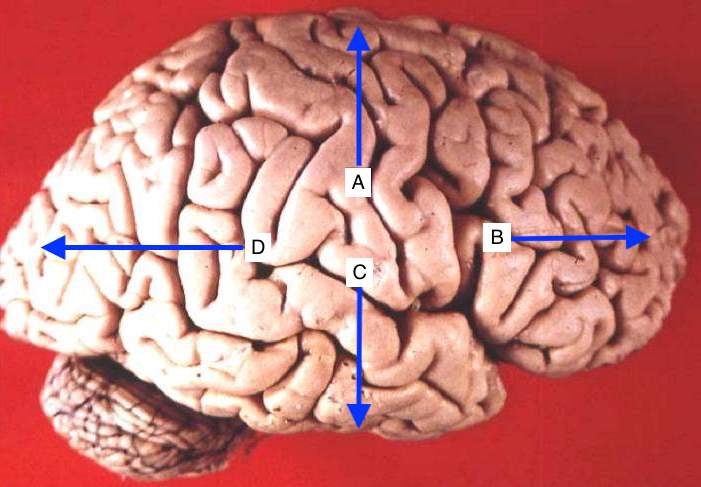
\includegraphics[scale = .25]{brain_directions.jpg}
\\b) Human Body (8 pts):\\
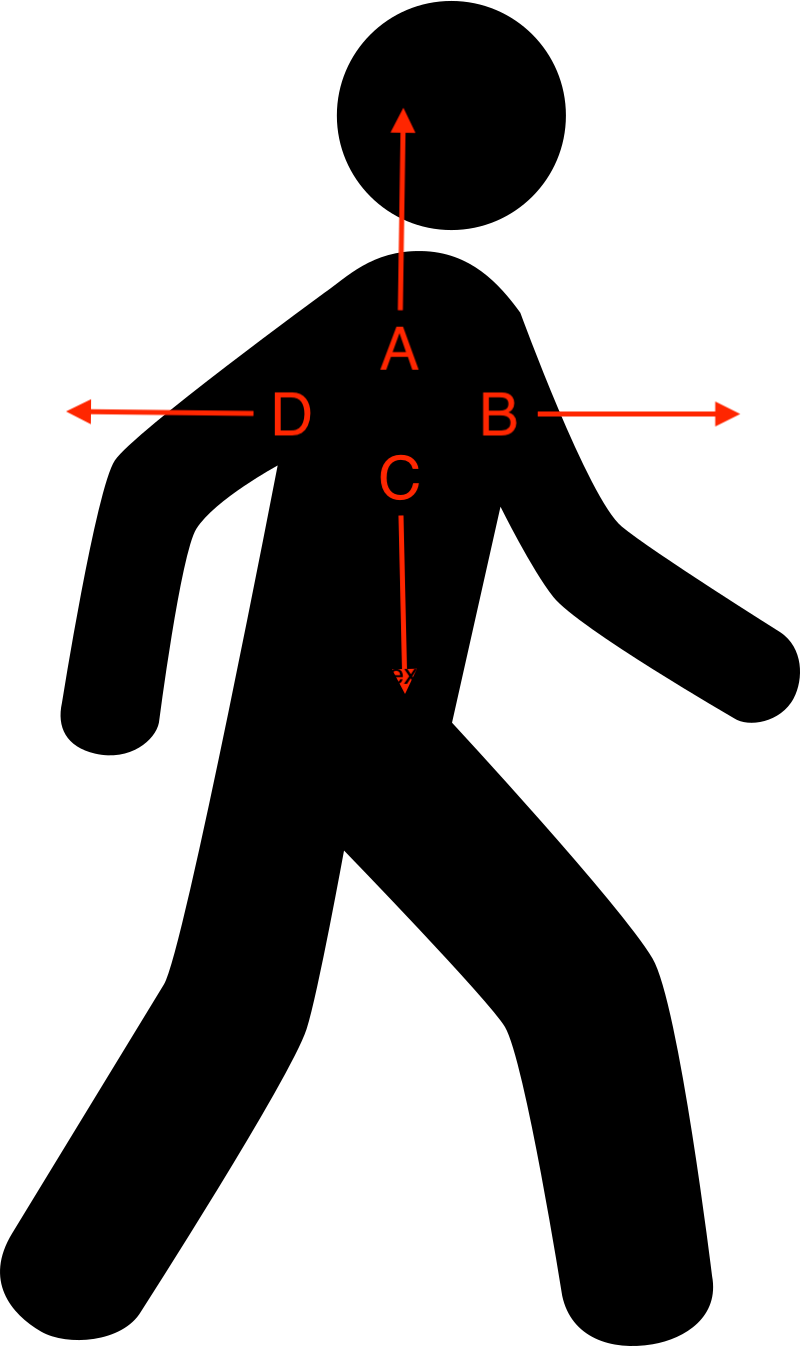
\includegraphics[scale = .12]{man.png}
\\c) Dog (8 pts):\\
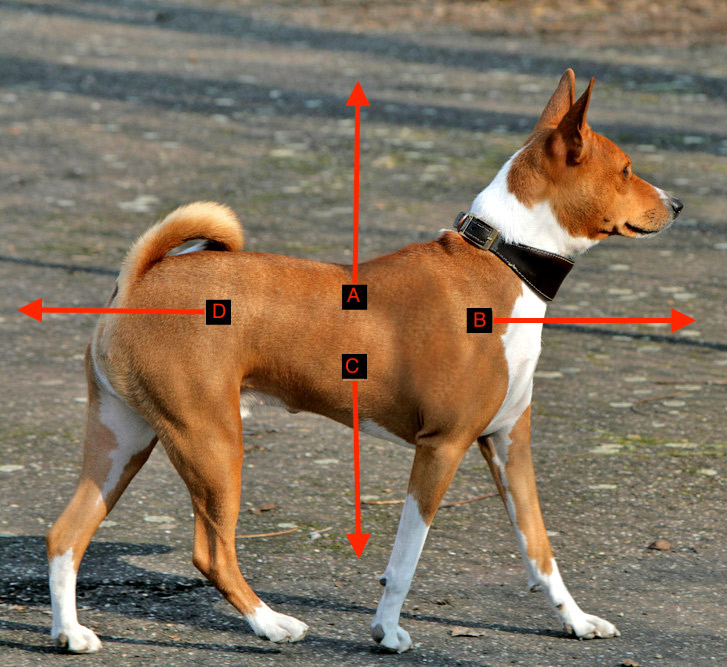
\includegraphics[scale = .23]{dog_directions.jpg}

\subsection*{Problem 5 (11 pts)}
According to the Goldman–Hodgkin–Katz equation, if the membrane were more permeable to Na+ at rest, instead of K+, what would the approximate resting membrane potential be?
\begin{enumerate} 
    \item[A.] –70 mV
    \item[B.]+50mV %this is the answer
    \item[C.]–79 mV
    \item[D.]+100mV
\end{enumerate}

\subsection*{Problem 6 (20 pts)}
For each of the following, indicate whether each condition would cause a hyperpolarization or depolarization of the membrane potential:\\

Increase in extracellular K$^+$ (5 pts):\\ %depolarization

Increase in Na$^+$ permeability (5 pts):\\ %depolarization

Increase in  K$^+$ permeability (5 pts):\\ %hyperpolarization

Increase in  extracellular Cl$^-$ (5pts):\\ %hyperpolarization, 2 points for slight/no change (full 4 for slight hyperpolarization)



\end{document}
